\chapter{Security of Android}
\label{chap:and-secu}

\section*{Introduction}
As the number of smartphones is in constant raise, the level of concerns about the security of the system increases.
Paradoxically, the users tend to store more and more personal data on their smartphones and are not aware of the security issues of such devices.
Malwares have been discovered on the official applications store and antivirus softwares for Android are now available.
Android runs on top of a Linux kernel which is yet reputed to be virus free.\\

The aim of this chapter is to explain in detail the current security mechanisms used to protect the users against malicious applications.
Using the presented information, a user should be able to reduce his infection risk by adopting simple security principles.
The focus of this chapter is the application capabilities and propagation.
Different security threads are examined and the risks associated are evaluated.
The different procedures from the publication to the installation of an application on a device are particularly examined.

The forensic aspect to retrieve information from a device without the owner consent have not been analysed here.\\

These clarifications are essentials to understand the limits and possibilities for the developed \emph{DroidWatcher} (see Chapter \ref{chap:droidwatcher}) application to be effective.

\section{Permissions}
\label{sec:permissions}

For an application to run on the Android operating system and access to critical resources, it should have explicitly been allowed to do so.
For a set of defined tasks, a permission should be enabled.
These tasks are, for example, accessing the current location of the user, update the address book, use the Internet, write to the SD card...
At the installation of an application, the permissions necessary are mentioned.\\

The permission system is designed to control the usage of internal methods and resources of Android.
Without a permission, an application can not access to certain resources or methods in the Android system.

\subsection{Technical details}
%In Appendix \ref{perm-list}, the list of available permissions are mentioned.
The full list of permissions with a brief description is available on the Android documentation\footnote{Available at \url{https://developer.android.com/reference/android/Manifest.permission.html}}
These permissions are defined in the configuration file \texttt{AndroidManifest.xml} present in every application.
Without the correct permission, an application throws an exception when the method accessing the forbidden resource is launched.

\begin{lstlisting}[breaklines,caption={Example of permission violation log},label={lst:gpsexception},numbers=none]
E/AndroidRuntime( 1274): FATAL EXCEPTION: main
E/AndroidRuntime( 1274): java.lang.RuntimeException: Unable to start activity ComponentInfo{com.example.gpstest/com.example.gpstest.MainActivity}: java.lang.SecurityException: Provider gps requires ACCESS_FINE_LOCATION permission
...
E/AndroidRuntime( 1274): Caused by: java.lang.SecurityException: Provider gps requires ACCESS_FINE_LOCATION permission
...
\end{lstlisting}

In Listing \ref{lst:gpsexception}, is shown the Android debugger trace of an application requesting the location of the device using the GPS location provider without having requested the \texttt{ACCESS\_FINE\_LOCATION} permission.
If the error is not caught properly, the execution of the application is interrupted and the users receives a notification of the crash of the application.\\

The permission processed is conceived to control the access to an information and not a phone characteristic.
For example, the \texttt{ACCESS\_COARSE\_LOCATION} permission is not limited to the usage of the high level \texttt{LocationManager} methods but is also required for an application to retrieve the surrounding cell towers information (as these towers have a unique identifier, this lower level information could also be used to locate the user\footnote{This method is used in the DroidWatcher application to estimate the location even when no network connectivity is available}).

\subsection{Weaknesses}

The way the permission system is implemented does not fully prevent malicious behaviours.
The permission description is unclear and can include different purposes.
For example, the permission \texttt{READ\_PHONE\_STATE} is required for many actions.
It allows an application to be notified when a phone call is processed or when the device is locked, it also gives information about the phone unique identifier and SIM id.
This permission is often used to suspend services or simply track a device using the unique identifier.
The problem is that, in case of a phone call, it also provides the access to methods allowing to retrieve the caller phone number.
This is an information leakage that could have been avoided.\\

Also, it is unclear when and why an application requires a permission at the installation process.
Many free applications display advertisements to fund their development.
This kind of applications requires the permission to access the Internet to download the advertisement content.
A malicious gaming application could justify the need for the two permissions \texttt{INTERNET} and \texttt{WRITE\_EXTERNAL\_STORAGE} (access the micro-SD card of the device) for advertising and score storing.
Using these permissions, it could upload the full content of the SD card (which may contains personal information from the other applications) to a server.
Only a deep analysis such as network monitoring can detect malicious behaviours of an application.\\

Finally, if a user disagrees with the need of a suspicious permission, it has no other choice than not installing the application.
There is no possibility to partially accept the permissions.
Due to this restriction, if they want to use the application, we can assume than most users will accept, whatever the asked permissions are.

\section{Installation of applications}

Unlike iOS where the App Store is the only permitted source of applications\footnote{Alternative markets and applications distributions exist on iOS but they require jail-breaking which is not allowed by Apple}, the Android operating system proposes several ways to install an application.

\subsection{Play Store}
By default\footnote{The Play Store is available only on official Android devices approved by Google. The Android operating system is open source which allows the port on many devices but the Android Play Store application is closed sources and compatible with only the official Android devices.}, the Android Play Store (formerly named Android Market before its merging with Google Music) is the only source of applications.
Once a Google account is associated to the user's phone, it can use the application Google Play Store which lists the available applications and install them quickly.
Figure \ref{fig:market} shows an example of the interface of the application.\\

\begin{figure}[h]
  \centering
  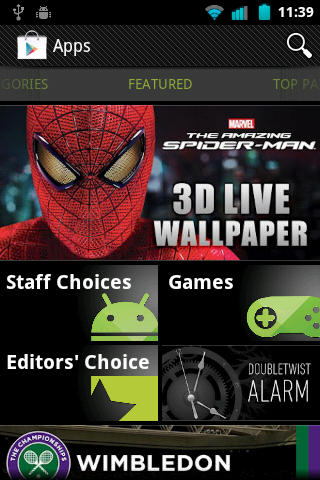
\includegraphics[width=4cm]{images/market1.png}
  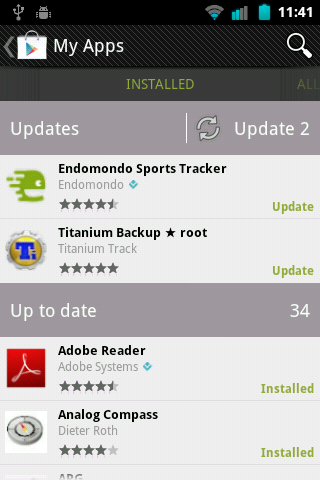
\includegraphics[width=4cm]{images/market2.png}
  \caption{Google Play Store interface}
  \label{fig:market}
\end{figure}

The Android Play Store has several features that can be handy for the average user:
\begin{itemize}
\item Warning when an update is available
\item Control by Google against malicious applications
\item User comments and review
\item Paid system with Google Checkout
\end{itemize}

On the website \url{https://play.google.com/store}, the content of the Android Play Store is available from a browser.
An important feature of this website is the possibility, once logged with the associated Google account, to select applications to install.
The next time the Android device is connected to the Internet, it will automatically download and install the selected applications without any user interaction required.
A simple notice is displayed on the phone once the application is installed.\\

%http://androidforums.com/android-applications/36936-android-permissions-explained-security-tips-avoiding-malware.html

\subsection{Other sources}
By default, the possibility to install applications from other sources than the Play Store is disabled.
Changing this setting is proposed when a user is trying to install a software from another source for the first time.

\subsubsection{.apk file}
The \emph{.apk} extension is the convention for installable applications on the Android operating system in the same way as \emph{.deb} or \emph{.rpm} are on Debian and Fedora operating systems.\\

A user trying to open such files on his device launches the installation process in the same way as if he was using the Android Play Store.
The required permissions are displayed and ask for the approval of the user.
Figure \ref{fig:perm-dw} shows the permission screen when a user tries to install the application DroidWatcher.
This is the same screen while using either the Google Play Store or installing an \emph{.apk} file.\\

\begin{figure}[h]
  \centering
  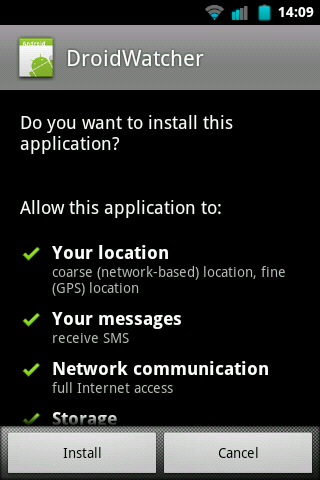
\includegraphics[width=5cm]{images/permissions.png}
  \caption{Permissions required to install DroidWatcher}
  \label{fig:perm-dw}
\end{figure}

An apk file is produced after the compilation of a program and is often proposed on small projects or for beta versions.
Once an application is installed on the system, the apk file is stored on the system.

\subsubsection{Alternative marketplace}
In the same way as the Android Play Store, it exists several alternative market places.
Alternative market places are a way to download apk files from a centralised interface.
It is seen as an alternative to the Google Play Store with the advantages of a centralised distribution medium (paid system, users reviews, moderation...).
Manufacturers or service providers sometimes sell smartphones with their own marketplace instead of the Google Play Store.\\

% TODO \emph{jesaispluslenom} on the other hand as a fewer control which leads to finding more malicious applications or pirated versions of non-free applications available on the Play Store.

\subsubsection{Debug mode}
If the debug mode of an android device is turned on (done in the configuration settings of the device), interaction between a computer and the device is possible.
Using the official Android Debug Bridge toolkit\footnote{Documentation \url{https://developer.android.com/tools/help/adb.html}}, an application can be installed in a few seconds from a computer without any notifications or user interactions on the device connected to a computer (connection done typically using a USB cable).
%The device does not need to be unlocked to allow the installation.

\section{Attack schemes}

As the multiple installation procedures make the propagation of application easier, it also allows abuses and permit the propagation of malwares.
Figure \ref{fig:secu-graph} presents the different possibilities for a malicious applications to propagate and be installed on a device.
The attack types are described in Section \ref{sec:malware-type}.

\begin{figure}[h]
  \centering
  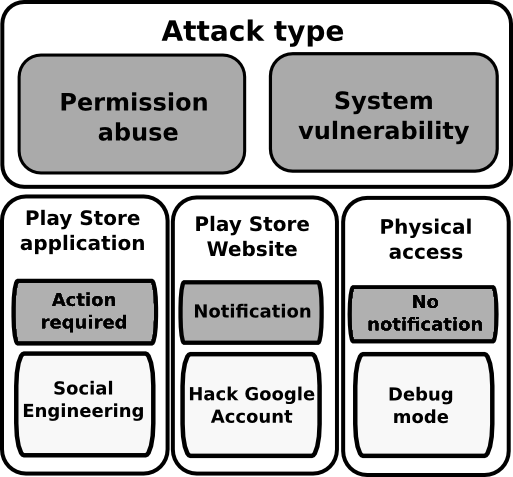
\includegraphics[width=8cm]{images/secu-graph.png}
  \caption{Malicious applications propagation possibilities}
  \label{fig:secu-graph}
\end{figure}

\subsection{Play Store publication policy}
\label{sec:playstore-publication-policy}

In comparison to the Apple iOS system, Google has adopted an open policy of application publication.
This strategy choice makes the Android system an easier target in term of malware propagation on the official applications distribution platform.\\

To distribute an application on the Android Play Store, the registered developer can upload his application on Google Play servers and make it available in a few hours\footnote{Official Distribution Control guidelines \url{https://developer.android.com/distribute/googleplay/about/distribution.html}}.
There is no human control before the publication of an application.
The upload of a malicious application would be detected only after its publication which can lead to infected users.
In comparison, when submitting an iOS application, Apple will review the application which can takes several days.\\

In February 2012, Google announced the creation of Bouncer, an automated scanning of the Android Play Store for potential malicious software.
This scan is applied on every new and already published application to detect known malwares, spywares and torjans or detected suspicious behaviour based on previous detection.
This prevents detected malicious applications to be republished on different developer accounts or under different names~\cite{secu-bouncer}.
However, in the 2012 DefCon conference, Bob Pan, from TrendMicro Inc. presented a way to bypass this security by dividing a known virus in several parts and recreate the infected apk afterwards~\cite{secu-defcon}.\\

To become a registered developer, the owner of a Google account has only to pay a 25\$ fee and no other information than a name and a phone number.
In comparison, to become a registered Apple developer, a minimum of 99\$/year fee\footnote{According to Apple Developer Programs \url{https://developer.apple.com/programs/}} to subscribe to the developer program is required and more personal information such as credit card information for identity verification.\\

This difference in the verification process and ease to create a developer profile between Google and Apple may lead to the presence of more malicious applications on the Android platform than on iOS.
The presence of an application on the Android Play Store is then, by no means, a guarantee of safety and a user should check carefully before installing any application.\\

As for the Play Store, alternative market places are as secured as the control of their owners over the applications acceptance process.
The \emph{Amazon AppStore}\footnote{Available in the US only at \url{http://www.amazon.com/appstore}} developed by Amazon.com Inc. has an approval process to publish applications similar to Apple regarding iOS applications\footnote{Approval Process and Content Guidelines \url{https://developer.amazon.com/help/faq.html\#Approval}}.

\subsection{Play Store website}

In the case of an attacker gaining access to the Google account of an Android user, it could remotely install any application.
This would allow the attacker to do almost any kind of actions the device is capable of.
It would be possible to monitor the activity of the user or remotely command the phone.
%The developed application \emph{DroidWatcher} is an example of what would be possible with a focus on the geolocalization.
A simple notification is displayed at the application installation that can be unnoticed or not understood as an infection sign by inexperienced users.

\subsection{Social engineering}

As the developer policy of Google is open by nature, the description of an application published on the Play Store may not describe the real behaviour of an application.
Free games or widgets are often attractive and are an ideal target for a malicious application writer that can use social engineering.
Pretending another purpose than the actual behaviour of an application leads to its installation willingly from the user.\\

This attack scheme is relevant for applications on the Play Store or installed using any other sources.
However, there is frequently a confusion from the users supposing the Play Store is more secure than it actually is.
This may lead to reduce the suspicion of the users and makes the attack more effective.\\

Also, websites have appear on the web proposing applications that are non-free on the Play Store.
These applications can be instead a malware or have been manipulated to inject malicious code in the original application.
Therefore, applications downloaded on such websites should be considered as are the warez websites on the Windows operating system: highly risky in term of malware propagation.

\subsection{Physical access}

If a malicious user has a physical access to a device, it can install an application from a computer using the \emph{adb} utility in debug mode.
The micro-USB connectivity is an European standard recommendation for smartphone connectivity.
It is then easy to connect any smartphone to a computer with this connectivity.
If the debug mode is enabled\footnote{The debug mode is required for any interaction between a computer and a smartphone}, there is no need to activate the phone which makes the presence of screen lock ineffective.\\

When a malicious application is installed using this method, no notification is displayed, the only detection possibility is the presence of the application in the installed applications list.\\

It is recommended to disable the debug mode when not required and use a screen lock to prevent modifying the phone settings.

\section{Malwares}

\subsection{General malware types}
\label{sec:malware-type}

There is two main types of Android malwares: abuse of permission or use of security flaws.\\

The first kind of malware takes advantage of the lack of suspicions from the users and simply ask for permissions allowing a malicious behaviour.
This is usually the case for applications sending text messages to overtaxed number or stealing contact information from the address book.
This kind of malware tends to be timeless and works as long as the users do not inspect attentively the permission screen whatever the operating system version he is running.
As some ``honest'' applications have a large range of features (that the user may never use), it is common to see such applications asking for many permissions (for example, the official Facebook application requires 19 different permissions\footnote{Discovered through personal researches by decompiling the downloaded application from the Android Play Store in July 2012}).
The reasons of the asked permissions is usually not mentioned by the application makers\footnote{Counterexample: Firefox browser created a page to explain the reason each permission is used \url{http://mzl.la/FirefoxPermissions}}.\\

The usage of security flaws is possible due to the slow update process.
The manufacturers tends to provide only a limited number of version updates if any\footnote{Computerworld has computed the percentage of Android phones upgraded to Froyo (released in May 2010) by each manufacturer within 2010 \url{http://blogs.computerworld.com/17649/android_upgrades}}.
A device older than a year is usually not maintained anymore.
The only solution for users owning such devices is to install alternative ROMs such as CyanogenMod that provides a longer support for a large range of devices.
When a security flaw is discovered and a patch published, only a very small percentage of users benefits from the patch through an update in the months following the discovery.
Malware writers can then wrote programs taking advantage of that flaw.\\

\subsection{The DroidDream malware}

In spring 2011, a malware named \emph{DroidDream} has widely spread across the Android devices.
The particularity of this malware was that he used the official Android Play Store (called Android Market at that time).
Referring to Figure \ref{fig:secu-graph}, it is classified as using social engineering to exploit a system vulnerability.\\

The attackers created several developers accounts and malicious applications (above 50 different applications were detected) on the Play Store.
The applications used social engineering by taking the name of popular applications and using modified versions of the application to trick the users into downloading them.
The malware used exploits effective until the version 2.2 (99\% of the devices at that time\footnote{Data collected based on the connections to the Android Play Store, source \url{https://developer.android.com/about/dashboards/index.html}}) to break the sandboxing mechanism, root the device and install other applications preventing the removal.
The malware has been called DroidDream as it was set up to run between 11pm and 8am to contact the master server.
Due to its ability to install other applications, the Kaspersky Lab's analysts suppose it could have been monetised in the future to be used as a botnet (spam sending, distributed denial of services...).\\

In reaction to the discovery of this malware, Google activated the \emph{kill switch} which deleted the malware from the user devices remotely.
It was the first known example of widely spread command-and-control malware on mobile devices.
Researchers estimated the number of infected users between 50,000 and 200,000 devices\footnote{According to the number of time the applications have been downloaded in total}.
Variants of this malware called DroidDream Lite have been detected a few months later.

\subsection{Protection}
Observing the large increase of malware applications on the Android platform\footnote{Between 2011 and 2012, the number of Android malware families has increased from 10 to 37 according to F-Secure \url{http://www.zdnet.com/blog/security/android-malware-families-nearly-quadruple-from-2011-to-2012/12171}}, users and developers wonder about the need of antivirus software.
As the antivirus for desktop computers works, these antivirus usually work using a malware database basis.
Such softwares would be efficient on antivirus using flaws and derived in several applications such as the DroidDream malware did.
However, on the second kind of malicious applications, the efficiency of the antivirus is mitigated as it is very easy and quick to develop applications abusing from the granted privileges.\\
%The open politic on the Google Play Store help the propagation of malwares as the users wrongly suppose a higher control (which is done instead by the users a posteriori).\\

\begin{figure}[h]
  \centering
  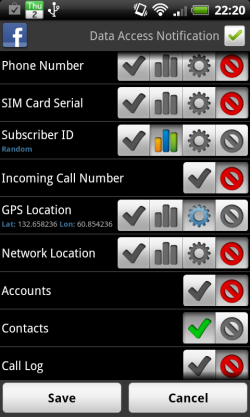
\includegraphics[width=6cm]{images/pdroid.png}
  \caption{PDroid on the Facebook application}
  \label{fig:pdroid}
\end{figure}


The PDroid application\footnote{Available on the xda-developers forum at \url{http://forum.xda-developers.com/showthread.php?t=1357056}} takes another approach than the antivirus softwares.
Instead of detecting the known malicious applications, it allows the users to redefine the granted permissions and revoking them at wish.
Another possibility instead of disallowing the access to certain information is to define a fixed or random value (eg: in the case of geographical coordinates).
For each application, a notification can be launched at the time the resource granted by a permission is used.
This feature can be useful to detect abuse of permissions.
However, as the PDroid application works as a intermediate layer between the operating system and the other applications, the application need the root privileges and the user has to apply a patch on the ROM files.
These requirements are most of the time not possible on manufactured phones with closed sources ROM and are reserved to users with good computer knowledge.
Although it is not applicable to most Android users, PDroid is a possibility of big improvement on the permission model and we can hope a similar model to be adopted in future versions of Android.
Figure \ref{fig:pdroid} is an example of usage of the PDroid application capabilities on the Facebook application.
